\chapter{Related Literature}

This chapter reviews some relevant literature and techniques that are referenced and utilized in this thesis. First, the basis behind guilds and the relevance to the human gut microbiome is discussed \citep{Goldford2018}.  Then the SparCC \citep{Friedman2012} and FastSpar \citep{Watts2018} algorithms will be introduced, followed by the case and control network comparison technique from NetShift \citep{Kuntal2018}. Additionally we mention the MicrobiomeHD project \citep{Duvallet2017} which contains the data used in this study.

%%%%%%%%%%%%%%%%%%%%%%%%%%%%%%%%%%%%%%%%%%%%%%%%%
\section{Emergent simplicity in microbial community assembly}\label{lit-gold}
As mentioned in the Background section, \citeauthor{Goldford2018}'s research revealed that there is conservation of microbial distributions across the family level in systems that have been allowed to grow to a stable state. \citeauthor{Goldford2018}'s motivation was to investigate whether taxonomic architectures can be explained and predicted by fundamental quantitative principles. Figure \ref{fig:rel-gold}
\begin{figure}[!thbp]
    \centering
    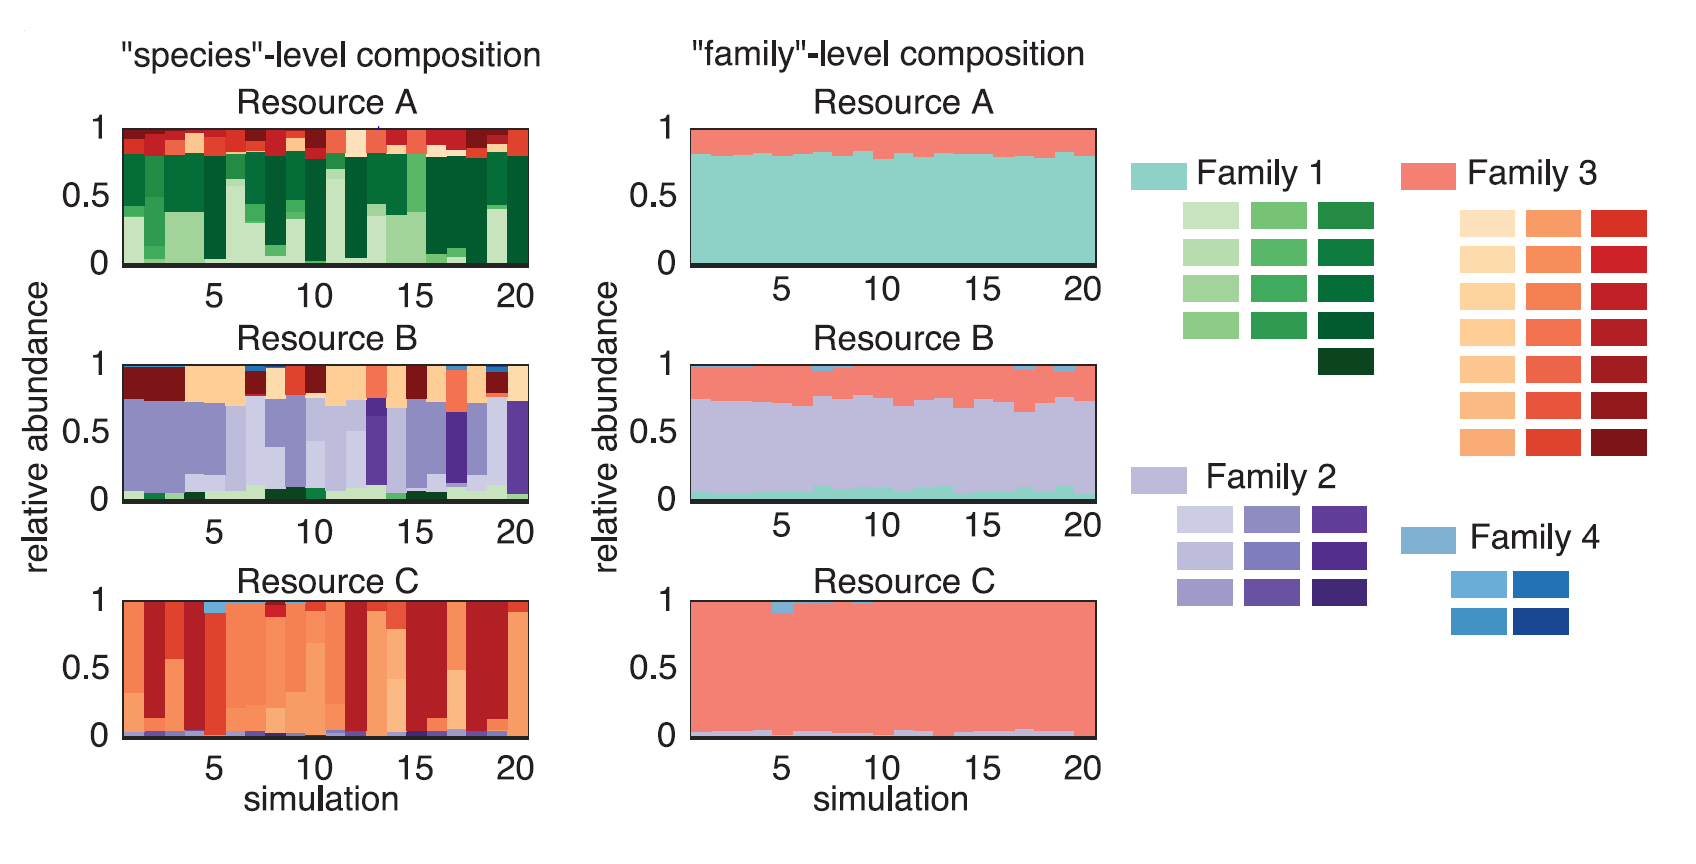
\includegraphics[width=0.95\linewidth]{figure/background/goldford_img.png}
    \caption[Community distribution plots from Goldford et al.]{Community distribution plots from \citeauthor{Goldford2018} The plots on the left look at the community composition at the species-level, and those on the right show the family-level composition. Family level composition is conserved across simulations and resource types. This image from \citep{Goldford2018} has been licensed for reuse in this thesis with permission from Science and The American Association for the Advancement of Science under the license number 4605400364700.}
    \label{fig:rel-gold}
\end{figure}
contains plots showing the composition at the species and family levels across 20 experiments with three different media present in the growth environments. 

Despite having the same initial populations and resource amounts, species level compositions at the stability point varied considerably, but the family level compositions remain conserved across studies. From these experiments and multiple other analyses, the authors determined that resources available to microbes significantly dictated the structure of a stable community. This type of behavior is not unique to the experiments, but can be extended to various other microbiomes such as the human gut, plant foliage, and oceans \citep{Goldford2018}. In general, the authors' work suggests that there are mechanisms that contribute to community-wide stability states. Part of this indicates that stabilized microbial communities consist of metabolic generalists instead of specialists, meaning that members of the communities carry certain functional roles. As they are swapped out for different microbes with similar roles, the overall behavior and family-level stability stays static.


\section{Sparse Correlations for Compositional Data}\label{lit-fastcc}

The \acrfull{SparCC} and \acrfull{FastSpar} methods are both very similar, but the latter has an improved $p$-value estimation. Together the techniques aim to take compositional data and treat counts as relative amounts. 

\subsection{Inferring Correlation Networks from Genomic Survey Data} \label{lit-sparcc}
This paper introduces the \acrshort{SparCC} method which was proposed by \citet{Friedman2012}. It was developed because genomic data gives relative, not absolute, abundances of the components of a community. The fact that the data is relative stems from the variabilities in sequence read depth and length. Metagenomics sequencing aims to resolve a general understanding of the taxonomic structure of a sample based upon high quality sequence reads. Therefore, absolute counts are not a given because many sequences are often filtered out based on quality. Common methods in the literature treat the compositional data as absolute and normalize observed counts by the total number of counts to get the fractional abundances. The problem here is that correlation estimates are biased since the fractions are not independent \citep{Buccianti2006} and the resulting correlations are based upon fractional relationships instead of the underlying biological processes \citep{Aitchison2003a,Friedman2012}.

\citeauthor{Friedman2012}'s analysis of standard correlation inference techniques concluded that it performs poorly on genomic data by looking at how the fractional abundance variation of one taxon greatly influences all of the other taxa in the opposite direction. This creates artificial positive and negative correlations based upon abundance values. To circumvent this the authors assume that the number of different taxa is large, and that the resulting networks are sparse. Their method takes the original abundances as basis variables and then assigns a fractional abundance based upon a sampling of a Dirichilet distribution of the basis variables. They then estimate the linear Pearson correlations between log-ratio transformed components. \citeauthor{Friedman2012} determined that their method is robust to violations of the sparsity assumption, does not unfairly treat rare taxa, is highly accurate on simulated data, and identifies phylogenetically structured correlations \citep{Friedman2012}.

The resulting correlation and statistical significance matrices represent fully connected networks that contain correlation connections in the range $[-1,1]$ for each possible \acrshort{OTU} pair. In the literature, authors tend to employ some type of threshold value to filter out unnecessary information and connections that may not be significant. This is most frequently done by modifying threshold values to obtain a network that is scale-free or meets some type of average path length or centrality measure, but even this is performed arbitrarily \citep{Perkins2009, Batushansky2016, Romero-Campero2016}. Following arbitrary threshold selection, \citeauthor{Friedman2012}  employ arbitrary thresholds when pruning the resulting networks to analyze. They selected edges greater than 0.3, and omitted unconnected nodes. Arbitrary threshold selection is neither right nor wrong, and the prevalence of truly scale-free network structures is a controversial topic in network science today \citep{Broido2019, Barabasi2018, Holme2019}. 

\subsection{FastSpar: rapid and scalable correlation estimation for compositional data} \label{lit-fastspar}

The \acrshort{FastSpar} method developed by \citet{Watts2018} takes the \acrshort{SparCC} method of \citeauthor{Friedman2012} and implements the algorithm in C++. The \acrshort{SparCC} program requires a great deal of memory and compute time for high dimensional data sets. The \acrshort{FastSpar} implementation was designed to decrease runtime of the \acrshort{SparCC} algorithm and to implement a less biased $p$-value calculation. Based upon \citeauthor{Phipson2010}'s paper, \citeauthor{Watts2018} argue that the $p$-value estimator in \acrshort{SparCC} is biased. To combat this they use a $p$-value estimation that corrects $p$-value understatement by allowing for the possibility that permutations of the data are repeated \citep{Watts2018, Phipson2010}. According to their results, \acrshort{FastSpar} was up to 821$\times$ faster with a memory reduction of up to 116$\times$ less than \acrshort{SparCC} using 16 threads, and also generated more accurate $p$-value estimations.

\section{‘NetShift’: a methodology for understanding ‘driver microbes’ from healthy and disease microbiome datasets}\label{lit-netshift}
The NetShift (network shift) methodology is proposed by \citet{Kuntal2018} to quantify the rewiring and changes in two different microbiome networks (defined as the case and control networks). The authors developed the \acrshort{NetShift} method so that they could generate biologically-backed inferences of microbiome interactions based upon the microbial interaction networks of the respective microbiomes. In order to perform a reasonable comparison between networks, \citeauthor{Kuntal2018} search for the shared nodes between the networks and extract all of the edges associated with them. The resulting sub-graphs are then analyzed to identify community-level changes which can identify key microbes in the networks, or network structure shift as defined by the authors. 

\citeauthor{Kuntal2018} quantify the overall changes in the networks by first looking at the Jaccard edge index (unique edges in a network compared to all of the edges in the two networks) and then running a hierarchical clustering algorithm to label communities based upon the network structure. They run the clustering on both the control and case networks, and then visualize the re-wiring of the network by tracking the community that each node is associated with in each clustering network. With this knowledge, the authors argue that one can identify significant community changes and identify specific microbes that are taking part in the community shuffling. While not referenced in the paper, this idea could be associated with the work of \citet{Goldford2018} and their ``guilds''. \citeauthor{Kuntal2018} then use a new metric to evaluate the changes in associations of a single node in the network which they call \acrfull{NESH}. \acrshort{NESH} is formally defined in Section \ref{theory:struct-change} and evaluates the neighborhood associations of each node. Nodes with high \acrshort{NESH} and betweenness are then considered to be ``drivers'' of the network. 

With the NetShift methodology we find microbes that may contribute to different community functionality and we can gain a better idea of the stability of the networks' structure between states. 

\section{Meta-analysis of gut microbiome studies identifies disease-specific and shared responses}\label{relate-meta}

Microbiome research has produced hundreds of studies linking human health and the human microbiome, but few try to leverage the statistical power of aggregating this data. \citet{Duvallet2017} performed a meta-analysis using 28 different studies which all contained control and case cohorts covering 10 different diseases. The authors were able to create a random forest model to classify healthy and diseased individuals solely using their microbiome sample. Such results suggest that there is inherent structure in the communities of healthy and diseased individuals regardless of the type of disease.

The meta-analysis included patients with the following health-disease states: \acrfull{ART}, \acrfull{ASD}, \acrfull{CD}, \acrfull{CIRR}, \acrfull{CRC}, \acrfull{EDD}, \acrfull{H}, \acrfull{HIV}, \acrfull{LIV}, \acrfull{MHE}, \acrfull{NASH}, \acrfull{OB}, \acrfull{PAR}, \acrfull{PSA}, \acrfull{RA}, \acrfull{T1D}, and \acrfull{UC}. Together these represent various types of diseases -- metabolic, neurological, cardiovascular, autoimmune, and other disease types. The binary classifier implemented by \citeauthor{Duvallet2017} reveal that health state is related to dysbiosis in the gut. Given this data, the authors also tried to build a multi-class classification model. The results were poor -- resulting in low accuracy measures. The failure to build a model for these disease types is probably attributed to the imbalance in classes and lack of sufficient data points to distinguish specific diseases from each other.  

The study by \citet{Duvallet2017} is an important first step in drawing conclusions from publicly available data. Going forward, the authors hope that the microbiome field will continue to make its data and associated patient metadata publicly available. A large concern of this study was batch effect, so future analyses should include additional disease types and data for the included studies in order to minimize potential batch effects. With additional data there should also be a better representation of possible microbiome states associated with the various diseases. 